\documentclass[../main.tex]{subfiles}
\graphicspath{{\subfix{../images/}}}
\begin{document}

% The Minion platform features six \ac{LiDAR} units providing both omnidirectional environmental awareness and forward-facing high-density perception.
% The \ac{LiDAR} suite is comprised of three Velodyne VLP-16 pucks and three Livox Horizon units.

% Three Velodyne VLP-16 \ac{LiDAR} sensors are positioned at aft-center, with the other two placed at approximately one-third intervals around the vessel at forward-port and forward-starboard, providing complete 360-degree coverage for navigation as well as object detection and avoidance.
% An additional three Livox Horizon solid-state forward-scanning \ac{LiDAR} sensors provide high-density measurements within the forward direction of motion.
Three Velodyne VLP-16 \ac{LiDAR} sensors are installed around the vessel to provide omnidirectional situational awareness. 
One unit is mounted near the aft-center position, and the other two are positioned at approximately one-third intervals around the forward-port and forward-starboard quadrants. 
Together, these sensors deliver nearly continuous 360° coverage for navigation and obstacle avoidance.

Each VLP-16 employs 16 lasers arranged in a vertical array that scans 16 distinct points elevation over its 30-degree vertical \ac{FOV} continuously over the 360-degree azimuth, producing approximately 300,000 \ac{pps} in single-return mode. 
The units are installed with a downward declination of approximately 5 degrees from the plane of the \ac{USV} deck to minimize blind-spots near the vessel's waterline.
As a result, one-half to one-third of their scanning azimuth is well above the horizon or pointing directly into the vessel and is discarded, drastically reducing the number of points each unit can publish.

% Both of these units are capable of approximately 1.4 million measurements per second.
% For an equivalent 80-degree horizontal FOV, the Velodyne’s effective $317,700 \text{ pts/sec}$ represents $\approx 22 \%$ of the overlapping \ac{FOV} of the Livox unit’s output.
% % While each Velodyne VLP-16 unit is capable of producing 300k \ac{pps} compared to the Livox unit's 280k, their 360-degree scanning pattern means that only 
% The principal distinction between them lies in their underlying scanning architectures and sampling density, which directly influences perception fidelity.
% The Velodyne VLP-16 LiDAR scans 16 discrete points spanning a 30-degree vertical \ac{FOV} emanating from the azimuthal plane of the device in a 360-degree horizontal \ac{FOV}that repeats identically with each rotation. 
% The points generated span the 360
% % To minimize blind spots near the base of Minion, each of the Velodyne units is mounted at a 15-degree declination from the vessel's deck plane, resulting in 
% These rings are notF
% % For vessels moving at typical speeds (2-5 m/s), platform displacement between rotations remains small relative to object size, resulting in near-perfect overlap of consecutive scans.
% At typical vessel speeds between $2 \text{to} 5 m/s$, successive Velodyne rotations overlap almost perfectly, causing sparse sampling of small or distant targets.
% % This means that small to medium-sized objects may not even be detected when at large distances from the sensor, as illustrated in Figure \ref{fig:LiDAR_scan_compare}.
% Consequently, small or distant targets may be undersampled or entirely missed in sequential Velodyne frames (Figure \ref{fig:LiDAR_scan_compare}).

In contrast, the three Livox Horizon solid-state \ac{LiDAR} units concentrate their scanning pattern within an $81.7 \times 25.1$ degree \ac{FOV}, generating up to 280,000 \ac{pps}. 
Although the nominal point rates are comparable, the Livox pattern can return $100 \%$ of its concentrated \ac{FOV} data. 
This higher spatial sampling density enables detection and classification of objects that may be smaller or further from the sensor.
A direct comparison of the discrepancy between the Velodyne and Livox scan patterns and point density is provided in Figure \ref{fig:LiDAR_scan_compare}.
The top-right image shows the dense point cloud of the Livox devices.
The light tower in the foreground and the large dock structure in the background can be seen in the camera view (left) and are both well defined in the red point cloud.
Two small buoys are also distinctly visible between the two structures.
In comparison, the point cloud returned by the Velodyne devices is shown in the bottom-right. 
The general form of the light tower can be seen; however, there are very few points returned from the large dock structure in the background, and the round buoys are undetected.

% The forward-scanning Livox devices operate differently, tracing a non-repetitive pattern across the \ac{FOV}.
% Two orthogonal mirrors oscillate at slightly different frequencies to cause the laser beam to trace a path that progressively fills the \ac{FOV} without repetition as shown in Figure ~\ref{fig:livox_scan_pattern}.

\begin{figure}[htbp]
\centering
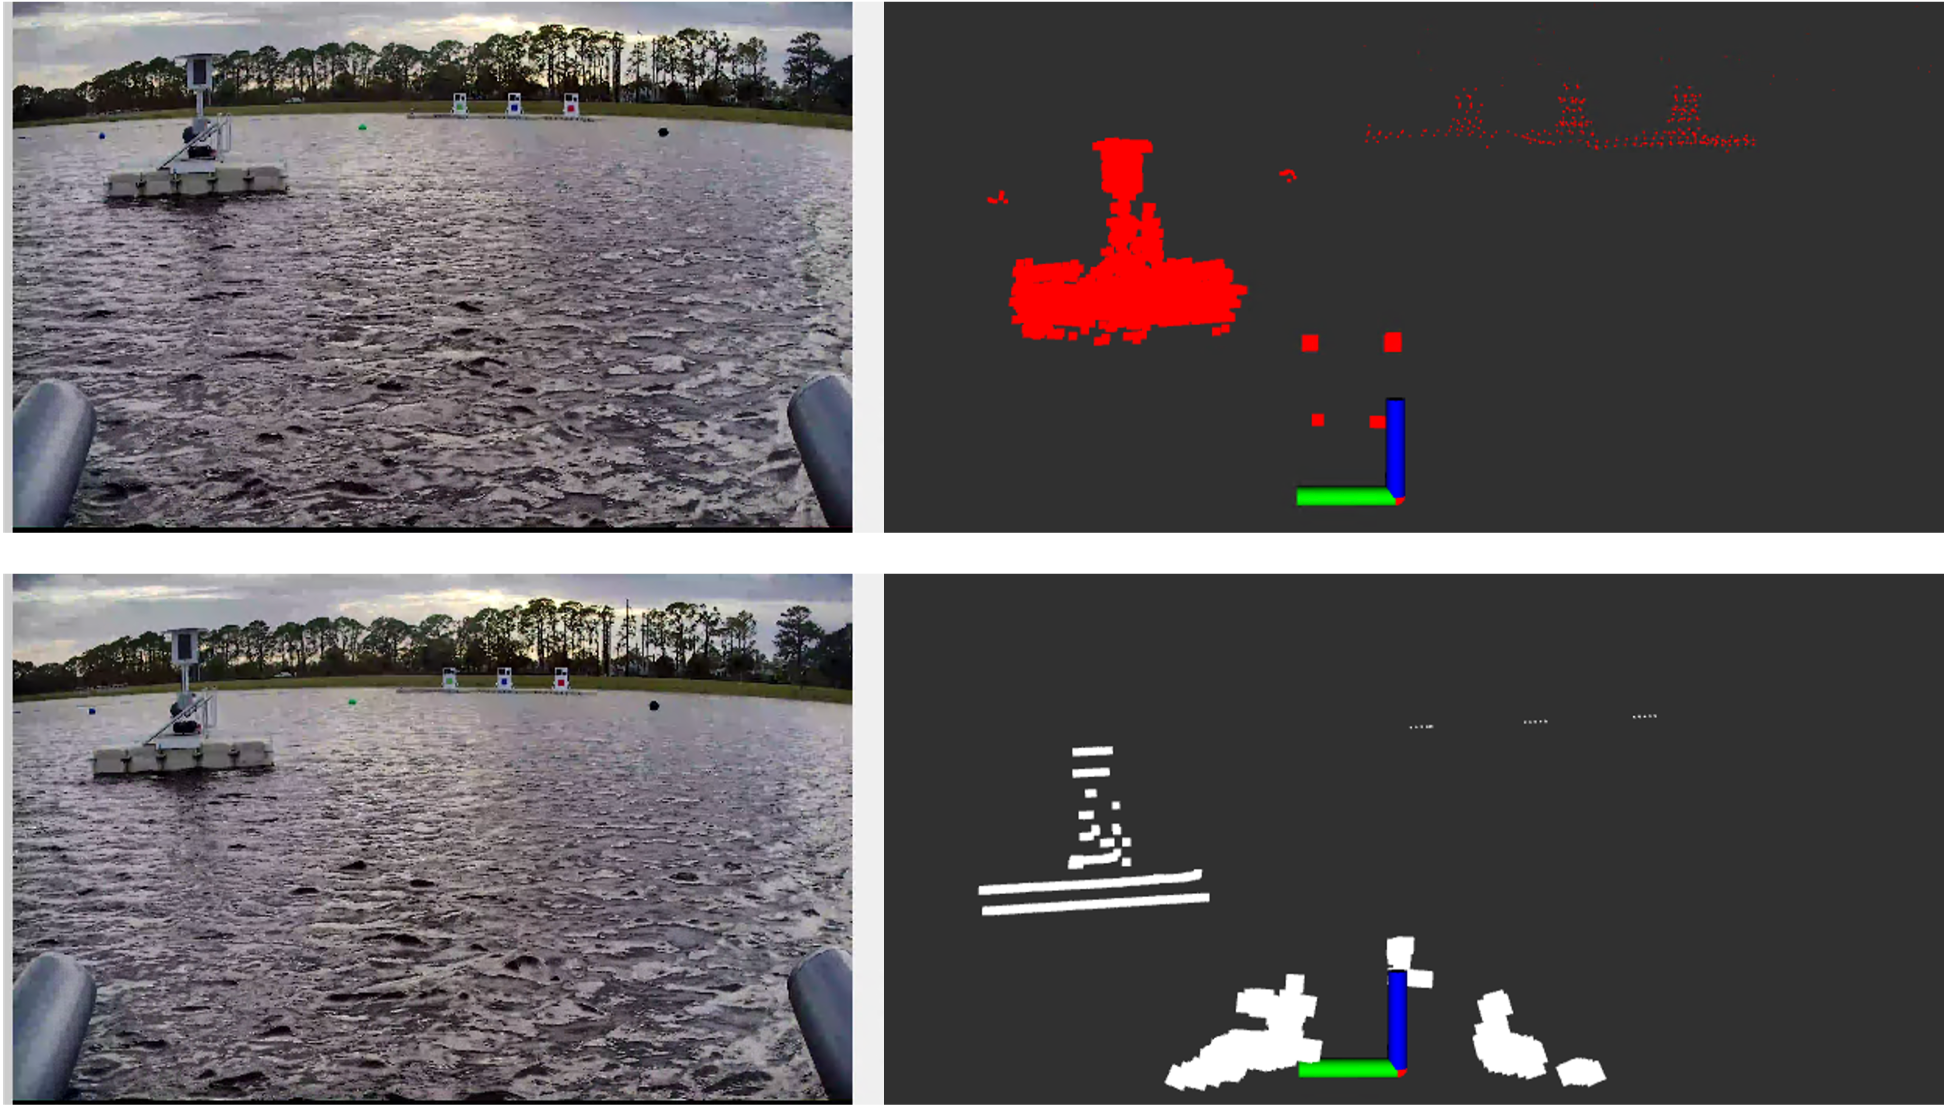
\includegraphics[width=0.8\textwidth]{Images/LiDAR_compare.png}
\caption{A comparison of LiDAR returns from the Livox units (top-right, red) and Velodyne units (bottom-right, white) to the respective HDR camera view (top-left and bottom-left). LiDAR points are viewed from third-person point of view in RVIZ. Green and Blue axes (top-right, top-bottom) represent the origin of the USV frame of reference.}
\label{fig:LiDAR_scan_compare}
\end{figure}

% The superior point density of the overlapping forward-scanning  LiDAR is critical for the real-time object detection method that is discussed in \textcolor{red}{Section \#}.
% The overlapping forward-scanning LiDAR provides the spatial density required for the real-time object-detection framework described in Section \ref{gbcache}.
% For this reason, the research presented in this work exclusively utilizes LiDAR data from the Livox Horizon sensors.

Consequently, the research presented in this work relies exclusively on LiDAR data from the forward-scanning Livox Horizon sensors, whose concentrated and non-repetitive coverage provides the spatial resolution required for the real-time object-detection framework described in Section \ref{gbcache}.
        %%%%%%%%%%%%%%%%%%%%%%%%%%%%%%%%%%%%%%%%%%%%%%%%%%%%%%%%%%%%
\subsubsection{Livox Horizon} \label{sensors_livox}

% Each Livox Horizon employs two orthogonal mirrors operating at different frequencies to trace a complex Lissajous-like path that progressively fills the $81.7 \times 25.1$-degree (horizontal × vertical) \ac{FOV}, as illustrated in Figure~\ref{fig:livox_scan_pattern}. 
% The three Livox units are mounted with 40 degrees of horizontal separation, overlapping each other \ac{FOV} by $\approx 50\%$, making the system robust to failure of any single unit, as well as effectively doubling the rate of sampled points and distributing them more evenly across the center device's \ac{FOV}. 
Each Livox Horizon uses dual orthogonal mirrors oscillating at slightly different frequencies to generate a non-repetitive Lissajous-like scan pattern over its $81.7 \times 25.1$ degree \ac{FOV}. 
Overlapping these sensors by roughly $50 \%$ effectively doubles the point density along the center-line path under nominal operation, and maintains coverage under single-unit failure.
Table~\ref{table:livox_horizon_specs} presents detailed hardware specifications for the Livox Horizon.

% The rosette scan pattern is provided in \ref{fig:livox_scan_pattern}, and table \ref{table:livox_horizon_specs} presents the Livox Horizon specifications.

\begin{figure}[htbp]
\centering
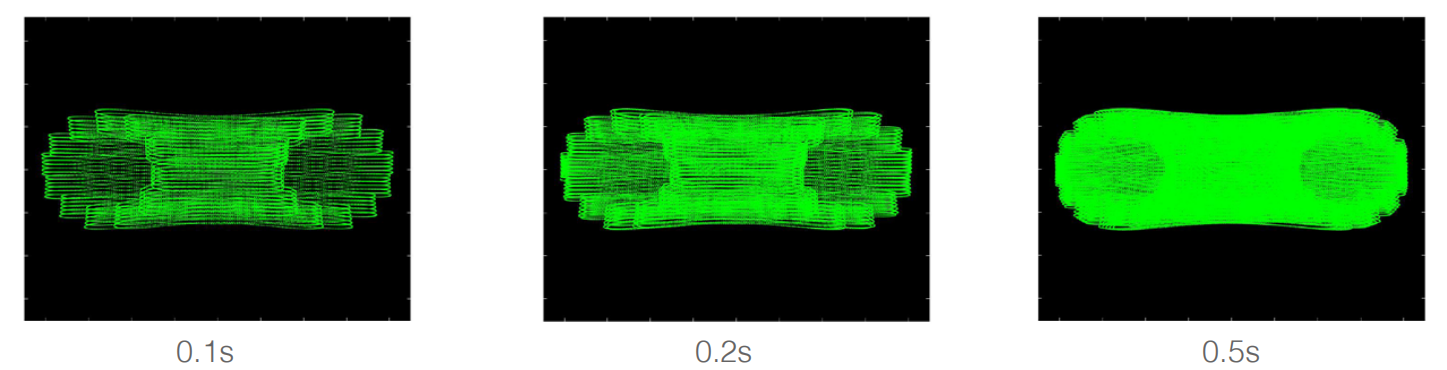
\includegraphics[width=0.8\textwidth]{Images/Livox_1.png}
\caption{Accumulation of points with the Livox Horizon's non-repetitive scan pattern, from 0.1 to 0.5 seconds  \cite{livox_manual}.}
\label{fig:livox_scan_pattern}
\end{figure}

Each device is capable of returning up to $4.8 \times 10^5$ \ac{pps} in dual return mode, with each return consisting of position coordinates (x, y, z), target reflectivity, and timestamp.
This operational mode returns two data points for each laser emission and is useful for situations where the sensor scans semi-permeable objects such as windows, thick tree canopies, or water.
% Instead, each device is operated in single-return mode for two reasons.
% The first is a consideration of available network bandwidth.
Each sensor operates in single-return mode, primarily to reduce network load.
A conservative estimate of 16 bytes per point results in $\approx 23 \text{ Mbps}$ which would quickly overwhelm the \ac{USV}'s network.
% Luckily, the 905 nm near-infrared wavelength of the emitted laser experiences strong absorption by water. 
However, The $905 nm$ near-infrared emission is strongly absorbed by water, effectively suppressing subsurface returns.
This means that only points which are reflected by the water surface are returned with an intensity greater than zero, making it straight forward to filter out points in the ground plane.

\begin{table}[htpb]
\centering
\begin{tabular}{ll}
\hline
\multicolumn{2}{c}{Livox Horizon}\\
\hline
% \textbf{Parameter} & \textbf{Value} \\
\hline
Model & Livox Horizon \\
Horizontal Field of View & 81.7 degree \\
Vertical Field of View & 25.1 degree \\
Range & 260 m @ 80\% reflectivity \\
Point Rate (Single Return) & 240,000 pts/sec \\
Point Rate (Dual Return) & 480,000 pts/sec \\
Range Precision & ±2 cm \\
Wavelength & 905 nm \\
Scan Pattern & Non-repetitive rosette \\
Interface & Ethernet \\
Operating Frequency & 100 Hz \\
\hline
\end{tabular}
\caption{LiDAR Specifications}
\label{table:livox_horizon_specs}
\end{table}

\end{document}